%% P6 manuscript for PFG - Journal of Photogrammetry, Remote Sensing and Geoinformation Science.
%% Revision 2 (18/10/2026) after internal review round 1 (paper_pfg/review/response_round1.md).
%% Every number is taken from the result files of code/s2sr_bench; the source is noted next to each table.
%% Numbers that do not appear in an experiment summary are in results/p6_paper_facts/facts.md.
%% Build: latexmk -pdf main.tex
\documentclass[pdflatex,sn-basic,referee,lineno]{sn-jnl}

\usepackage{graphicx}
\usepackage{amsmath,amssymb}
\usepackage{booktabs}
\usepackage{multirow}
\usepackage{xcolor}

\newcommand{\rreg}{r_{\mathrm{reg}}}
\newcommand{\HP}{\mathrm{HP}}

\begin{document}

\title[Imperfect cross-sensor references for Sentinel-2 super-resolution]{Imperfect cross-sensor references for
Sentinel-2 super-resolution: hidden benchmark errors and their consequences for training and evaluating deep
networks}

\author*[1]{\fnm{Cao Vu} \sur{Bui}}\email{vubc@fe.edu.vn}
\author[2]{\fnm{Hoang-Anh-Vu} \sur{Nguyen}}\email{vunha2@fe.edu.vn}
\affil*[1]{\orgdiv{Department of Artificial Intelligence}, \orgname{FPT University}, \orgaddress{\city{Da Nang}, \country{Vietnam}}}
\affil[2]{\orgdiv{Department of Computing Fundamentals}, \orgname{FPT University}, \orgaddress{\city{Da Nang}, \country{Vietnam}}}

\abstract{Airborne imaging spectroscopy provides high-resolution references for the 20\,m bands of
Sentinel-2, enabling supervised training and evaluation of super-resolution networks. These cross-sensor
references are harmonised to Sentinel-2, and their errors have not been characterised. Analysing
2,100 tiles of the SEN2NEON benchmark, we find a per-tile misregistration of the 20\,m bands (median 0.32 pixels at
10\,m), 131 tiles with resampled 20\,m inputs, and a contrast compression of the reference to 53--63\,\% of the
Sentinel-2 contrast: the harmonisation regresses Sentinel-2 on the airborne image, which turns any imperfect
correlation into lost contrast. After excluding the resampled tiles, a per-tile registration and one compression
factor per tile and band compensate these errors; on the 10\,m bands, where Sentinel-2 itself provides the truth,
this raises the detail amplitude of the reference from 0.62 to 0.82 of Sentinel-2. Training on the released
references lowers structural fidelity, and evaluating against them changes the ranking of methods under
amplitude-sensitive metrics (Kendall $\tau=0.53$ in simulation; on real data, models trained on uncorrected
references score highest by high-pass PSNR but lowest among supervised models by high-pass correlation). On nine
real test sites, training on corrected references raised the high-pass correlation by 0.043 (0.035 against the
reference as released). Among models trained on real references, a gain-invariant high-pass loss gave the best structure
and consistency with the observed 20\,m bands, but lower reduced-scale fidelity. Shift-tolerant losses,
privileged-information distillation and, within a fixed step budget, simulation pre-training did not improve on
plain L1.}

\keywords{Sentinel-2, super-resolution, deep learning, reference data quality, cross-sensor harmonisation,
image registration}

\maketitle

%% German abstract required by PFG (editorial template). DRAFT, to be checked by a German speaker.
\noindent\textbf{Zusammenfassung}\quad Hochaufgelöste Referenzen für die 20-m-Kanäle von Sentinel-2 (Red Edge,
schmales Nahinfrarot und kurzwelliges Infrarot) sind seit Kurzem durch flugzeuggestützte bildgebende Spektroskopie
verfügbar und ermöglichen das überwachte Training und die Bewertung von Super-Resolution-Netzwerken für diese Kanäle.
Die Referenzen entstehen durch sensorübergreifende Simulation und radiometrische Harmonisierung; ihre Fehler wurden
bisher nicht untersucht. In 2.100 Kacheln des SEN2NEON-Benchmarks finden wir eine Fehlregistrierung der
20-m-Kanäle pro Kachel (Median 0,32 Pixel bei 10\,m), 131 Kacheln mit resampelten 20-m-Eingangsdaten und eine
Kompression des Referenzkontrasts auf 53--63\,\% des Sentinel-2-Kontrasts (Mediane): Die Harmonisierung regressiert
Sentinel-2 auf das Flugzeugbild und wandelt so jede unvollständige Korrelation in Kontrastverlust um. Nach Ausschluss
der resampelten Kacheln kompensieren eine Registrierung pro Kachel und ein Kompressionsfaktor pro Kachel und Kanal
diese Fehler im angenommenen Degradationsmodell; in den 10-m-Kanälen, für die Sentinel-2 selbst die Wahrheit
liefert, erhöht die Kompensation die Detailamplitude der Referenz von 0,62 auf 0,82 der Sentinel-2-Amplitude. Das Training mit
den unveränderten Referenzen verringert die strukturelle Genauigkeit, und die Bewertung mit ihnen verändert die
Rangfolge der Methoden bei amplitudenabhängigen Maßen. Auf neun realen Testgebieten erhöhte das Training mit
korrigierten Referenzen die Hochpasskorrelation um 0,043; gemessen an der unveränderten Referenz betrug die Erhöhung
0,035. Ein
verstärkungsinvarianter Hochpassverlust lieferte die beste Struktur und unter den mit realen Referenzen trainierten Modellen die beste
Konsistenz mit den beobachteten 20-m-Kanälen, jedoch eine geringere Genauigkeit im reduzierten Maßstab
(Wald-Protokoll). Verschiebungstolerante Verluste, Destillation privilegierter Information und Vortraining auf Simulationen
verbesserten das einfache L1-Training mit korrigierten Referenzen nicht.

\section{Introduction}\label{sec:intro}

The Multispectral Instrument of Sentinel-2 observes four bands at 10\,m and six bands at 20\,m: three red-edge
bands (B5--B7), a narrow near-infrared band (B8A) and two short-wave infrared bands (B11, B12)
\citep{drusch2012sentinel2}. Bringing the 20\,m bands to 10\,m with the help of the 10\,m bands, a guided
super-resolution (SR) problem, is a long-standing task with model-based \citep{brodu2017supres} and deep-learning
solutions \citep{lanaras2018dsen2,aybar2026sen2sr}. Because no sensor observes these bands at 10\,m, deep networks
have mostly been trained and evaluated at a reduced scale: the 20\,m bands are degraded to 40\,m, the 10\,m bands to
20\,m, and the network learns to recover the original 20\,m bands \citep{wald1997fusion,lanaras2018dsen2}. Whether
what is learned at 40$\to$20\,m transfers to 20$\to$10\,m is assumed, not measured.

Real references would close this gap. SEN2NEON \citep{donike2026sen2neon} provides them for all Sentinel-2 bands:
AVIRIS-NG imaging spectroscopy from the NEON airborne observation platform \citep{hamlin2011aviris,kampe2010neon}
is convolved with the Sentinel-2 spectral responses, resampled to 2.5\,m and radiometrically harmonised to the
Sentinel-2 acquisition closest in time. To our knowledge it is the first openly available reference at sub-10\,m
resolution for the red-edge and short-wave infrared bands. The dataset is released as a benchmark, and it is
natural to use it also to train networks on real Sentinel-2 inputs.

A cross-sensor reference is not an error-free observation of the target sensor. It differs from what Sentinel-2 would have recorded at 10\,m through
registration, radiometric harmonisation, the point-spread function and surface change between acquisitions, which
are up to 40 days apart in SEN2NEON. \citet{michel2025revisiting} showed that geometric and radiometric distortions
of cross-sensor references bias SR metrics, and losses that tolerate misalignment have been proposed for natural
images \citep{mechrez2018contextual,zhang2019zoom,ni2024fdl,elezabi2024mimicked}. What is missing for Sentinel-2 is
(i) a measurement of the errors of the reference that is actually used, (ii) an understanding of where they come
from, and (iii) evidence of what they do to training and to evaluation, together with the training strategy that
copes with them best.

This paper addresses these three points for SEN2NEON. Its contributions are:
\begin{enumerate}
\item A characterisation of the reference errors on 2,100 tiles (Sections~\ref{sec:method-errors} and
\ref{sec:res-errors}): a per-tile translation of the target bands (median 0.32 pixels at 10\,m), local residuals
that grow with the time between acquisitions, and 131 tiles whose 20\,m input bands were resampled and are
therefore not native 20\,m data.
\item The mechanism of a contrast compression of the reference. The harmonisation regresses the interpolated
Sentinel-2 image on the airborne simulation and keeps the fitted values; by the attenuation mechanism of regression
dilution \citep{frost2000dilution} this shrinks the reference contrast whenever the two images are imperfectly
correlated. We verify the mechanism on every tile, compensate it with one compression factor per tile and band, and
validate the compensation in simulation, across spatial scales and on the 10\,m bands, for which Sentinel-2
observes the truth.
\item Evidence, in a simulation where the target is known by construction and on real data, that the uncorrected reference harms
training and changes the ranking of methods when they are evaluated with amplitude-sensitive metrics
(Sections~\ref{sec:res-controlled} and \ref{sec:res-real}).
\item A comparison of training strategies with a common student and student-step budget, with pre-specified hypotheses, three seeds for
every real-data method and site-level statistics on real data: plain, shift-tolerant, contextual, frequency and gain-invariant high-pass losses,
privileged-information distillation and simulation-based pre-training; ten strategies in simulation and nine on
real data (Table~\ref{tab:methods}).
\end{enumerate}
Fig.~\ref{fig:overview} summarises the study. Two of our pre-specified hypotheses were not supported; we report
them as such and separate the one post-hoc analysis from the confirmatory results. We release code, the site split,
the tile shifts and gains, the corrected references and the evaluation protocol.

\begin{figure}[t]
\centering
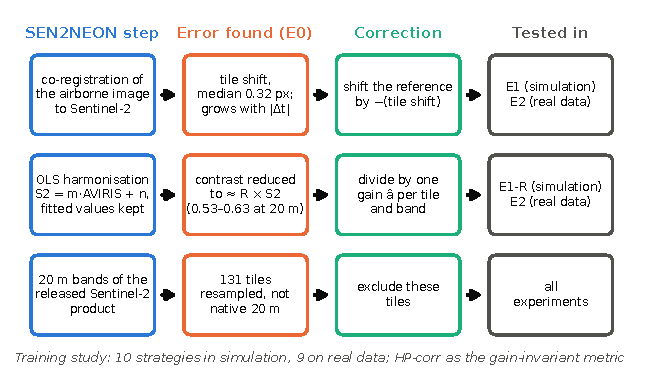
\includegraphics[width=\textwidth]{figures/fig1_overview.pdf}
\caption{Overview of the study. Each row follows one error of the SEN2NEON reference from the processing step that
causes it, through what the error analysis (E0) found and how it is corrected, to the experiments that test its
consequences in simulation, where the target is known by construction (E1, E1-R), and on real data (E2).}
\label{fig:overview}
\end{figure}

\section{Related work}\label{sec:related}

\subsection{Super-resolution of the Sentinel-2 20\,m bands}

Bringing the red-edge, narrow near-infrared and short-wave infrared bands to 10\,m is a guided SR problem: the
four 10\,m bands carry the geometry that the 20\,m bands lack. Model-based methods exploit this shared geometry
explicitly, for instance by assuming that the bands share the same sub-pixel structure \citep{brodu2017supres}.
Deep networks have largely replaced them. DSen2 \citep{lanaras2018dsen2} trained a residual network on globally
sampled reduced-scale pairs (40$\to$20\,m) and showed that it generalises across climate zones; later work proposed
faster networks \citep{gargiulo2019fast}, residual dense \citep{salgueiro2021rdsr} and hierarchical fusion
architectures \citep{wu2023hfn}, and multiobjective training that balances the synthesis property of Wald's protocol
with the consistency of the output with the observed bands through the sensor MTF \citep{vasilescu2023multiobjective}.
Self-supervised and unrolled networks avoid external training data and fit the degradation model of each image
\citep{qian2023selfs2,nguyen2023unrolling}. SEN2SR \citep{aybar2026sen2sr} trains on harmonised synthetic data and
adds a hard low-frequency constraint so that the degraded output reproduces the observed bands, which removes
reflectance drift by construction; we use this constraint in all our models. Whatever the architecture, these methods
are trained and, except for SEN2SR, also evaluated at the reduced scale or on simulated data, because no 10\,m
observation of the 20\,m bands exists.

\subsection{Reduced-scale training and the scale-invariance assumption}

Wald's protocol \citep{wald1997fusion} degrades all bands by the resolution ratio, so that the original
coarse bands become the reference. Its central assumption, that performance is independent of scale, has long been
questioned in pansharpening. \citet{carla2015fullscale} extrapolated quality measured at several degraded scales to
the full scale because the assumption may fail depending on sensor and scene; the critical comparison of
\citet{vivone2015critical} assessed methods under both reduced- and full-resolution protocols and discussed their
consistency; and
\citet{ciotola2022fullres} reported that networks trained at the reduced scale are often disappointing at full
resolution and proposed full-resolution training with consistency losses instead. \citet{alparone2023fullscale}
traced contradictions between the two kinds of assessment to residual misregistration between the input images, a
mechanism that also appears in our results. For the Sentinel-2 20\,m bands, the size of the scale gap had not been
measured against a real 10\,m reference; our controlled and real experiments quantify it.

\subsection{Cross-sensor references for Sentinel-2 super-resolution}

Real high-resolution references for Sentinel-2 come from other sensors. They were first used for the 10\,m bands:
\citet{galar2020real} trained networks with a spectrally similar satellite as reference, \citet{salgueiro2020esrgan}
used WorldView imagery, and \citet{latte2020planetscope} PlanetScope, normalising its radiometry jointly with the
super-resolution. Public datasets followed: SEN2VEN$\mu$S \citep{michel2022sen2venus} pairs Sentinel-2 with
same-day VEN$\mu$S images at 5\,m for eight bands; WorldStrat \citep{cornebise2022worldstrat} pairs SPOT 6/7 with
multiple Sentinel-2 revisits; MuS2 \citep{kowaleczko2023mus2} uses WorldView-2 for multi-image SR; SEN2NAIP
\citep{aybar2024sen2naip} pairs Sentinel-2 with aerial NAIP images and derives a degradation model from them; and
multi-temporal and diffusion-based methods were evaluated against such references
\citep{tarasiewicz2023deepsent,donike2025diffusion}. For the 20\,m bands, references are rarer:
\citet{major2025holistic} combined real references for the 10\,m bands with synthetic pairs for the 20\,m bands, and
\citet{li2020planetscope} sharpened both groups with PlanetScope while showing that surface change between
acquisitions degrades the result. SEN2NEON \citep{donike2026sen2neon} is, to our knowledge, the first open
reference for all bands including the short-wave infrared, obtained from airborne imaging spectroscopy.
Building such datasets requires temporal matching, co-registration and radiometric adjustment
\citep{malczewska2023datasets}, and each step leaves residual errors. \citet{michel2025revisiting} showed on
SEN2VEN$\mu$S and WorldStrat that the remaining geometric and radiometric discrepancies bias common image quality
metrics, proposed frequency-domain and distortion metrics, and a training and evaluation strategy that is robust to
them. Our study is complementary: we identify a specific systematic error of the harmonisation itself, explain it,
correct it, and quantify its consequences for training as well as evaluation.

\subsection{Geometric and radiometric consistency of Sentinel-2 and cross-sensor data}

Sentinel-2 products are not perfectly co-registered: before the Global Reference Image was introduced,
multi-temporal misregistration reached more than one 10\,m pixel \citep{yan2018s2misreg}, sub-pixel phase correlation
revealed shifts between Sentinel-2 and Landsat-8 as well as between Sentinel-2 acquisitions \citep{skakun2017coreg},
and the Global Reference Image reduced the Sentinel-2 to Landsat co-registration error to below 6\,m (CE90)
\citep{rengarajan2024coreg}. Within a Sentinel-2 image, band-to-band misregistration also occurs, notably for moving
or elevated objects \citep{skakun2017bandmisreg}. Harmonised products such as HLS \citep{claverie2018hls} combine
co-registration, BRDF normalisation and spectral bandpass adjustment by linear regression between sensors.

Radiometric harmonisation by regression has a long history in relative radiometric normalisation, where an image is
mapped onto a reference with a linear fit \citep{yuan1996comparison}. The direction of that fit matters: ordinary
least squares treats one image as error-free, whereas orthogonal regression treats both symmetrically, and
\citet{canty2004normalization} compared the two for automatic normalisation; \citet{syariz2019orthogonal} used a
constrained orthogonal regression to preserve spectral consistency. In statistics, the attenuation of an OLS slope
when the regressor is noisy is known as regression dilution \citep{frost2000dilution}. To our knowledge, the
consequence of this choice for a super-resolution reference, where the fitted values replace the high-resolution
image and so inherit a contrast reduced by the correlation, has not been described.

\subsection{Learning from misaligned or imperfect references}

In computer vision, real-world SR datasets are built by registering pairs taken at different focal lengths, and the
residual misalignment limits pixel-wise training \citep{cai2019realsr}. Losses that tolerate misalignment compare
feature distributions with a spatial penalty, as the contextual and contextual bilateral losses do
\citep{mechrez2018contextual,zhang2019zoom}, or compare feature spectra \citep{ni2024fdl}; HighRes-net
\citep{deudon2020highresnet} scores predictions after the best shift within a small radius; Mimicked Alignment
\citep{elezabi2024mimicked} synthesises an input aligned with the reference during training; and
\citet{gupta2022unaligned} handle a misaligned guide rather than a misaligned target. In Earth observation, errors
in training data are common and seldom reported \citep{elmes2020training}, and the evaluation of deep models is
inflated when training and test data are spatially dependent \citep{kattenborn2022autocorrelation,karasiak2022spatial},
which is why we split by site. These works address random or geometric errors; a systematic, scene-dependent gain
error of the reference, which no shift or distribution matching removes, has received little attention.

\subsection{Privileged information and distillation}

Learning using privileged information \citep{vapnik2009lupi} uses data that are available only at training time;
generalised distillation \citep{lopezpaz2015unifying} casts it as a teacher--student problem. PISR \citep{lee2020pisr}
applied it to SR with a teacher that sees the high-resolution image and a variational information distillation
loss \citep{ahn2019vid}; contrastive representation distillation \citep{tian2019crd} is an alternative. A cross-sensor
reference available only for some training tiles is a natural privileged signal, which motivated the distillation
strategies of this study.

\section{Data}\label{sec:data}

\paragraph{SEN2NEON.} The dataset \citep{donike2026sen2neon} (CC-BY-4.0) contains 2,269 tiles of 2.56\,km from 49
NEON sites in the United States, acquired in 2018--2024. Each tile holds a Sentinel-2 L2A image on a 10\,m grid
($256\times256$ pixels, 20\,m bands stored as $2\times2$ replicas) and the harmonised AVIRIS-NG reference for the
same bands at 2.5\,m. The time between the airborne and the Sentinel-2 acquisitions, $|\Delta t|$, is at most 40
days (median 23). All tiles are labelled as validation data: the dataset was released as a benchmark rather than as
a training corpus, so our training use is a deliberate departure that we handle with a site split.

\paragraph{Notation.} For a tile, $g\in\mathbb{R}^{4\times H\times W}$ are the 10\,m bands (B2, B3, B4, B8),
$x\in\mathbb{R}^{6\times H/2\times W/2}$ the native 20\,m target bands (B5, B6, B7, B8A, B11, B12; one pixel of
each $2\times2$ replica block, after checking that the blocks are constant) and $r\in\mathbb{R}^{6\times H\times W}$ the reference aggregated from 2.5 to 10\,m with a Gaussian
kernel matched to the Sentinel-2 modulation transfer function (MTF) at Nyquist (0.29 for B5--B8A, 0.195 for B11
and B12, 0.24 for the 10\,m bands; ESA data quality report, December 2022). Each kernel is a Gaussian whose transfer function equals
the ESA value at the Nyquist frequency of the coarser grid, $\sigma = (k/\pi)\sqrt{-2\ln\mathrm{MTF}}$ fine pixels
for a factor $k$, followed by decimation; pixel-aperture integration is not modelled separately. The 10\,m target
is therefore an algorithmic product whose MTF at the 10\,m Nyquist frequency equals the native-band value and whose
degradation reproduces the observed 20\,m bands, $D(y)\approx x$; it is not a physical Sentinel-2 observation. In
this cascade the reference degraded to 20\,m has an MTF of about 0.21 (B5--B8A) and 0.13 (B11, B12) at the 20\,m
Nyquist frequency instead of 0.29 and 0.195, i.e.\ it is slightly smoother than the native bands at the finest
20\,m scales; at the scales of $\sigma\ge60$\,m used for the gain estimate the difference is negligible. $D(\cdot)$
denotes this degradation for a factor of two (10 to 20\,m). We write $r$ for the 10\,m aggregate of the released
reference, $\rreg$ for $r$ after registration, $y_c$ for the corrected reference (Section~\ref{sec:correction}) and
$y$ for the 10\,m target, which is known only in simulation. Between MTF values lowered and raised by 0.05, the
median target shift differed by 0.005 pixels and the median contrast gain by at most 0.001 (419 reliable tiles of a
454-tile subset).

\paragraph{Filtering.} A tile was excluded when more than 1\,\% of its $2\times2$ blocks in the target bands were
not constant, i.e.\ the 20\,m bands had been resampled (131 tiles; using them would feed interpolation artefacts into the
input and violate the 20\,m sampling model); when less than half of its pixels were valid
(28 tiles); or when the phase-correlation peak of the guide bands was below 0.1 (10 tiles). The remaining 2,100
tiles enter the error analysis. Cloud contamination is described by the per-tile Cloud Score+ value provided in the
SEN2NEON metadata; radiometric statistics use the tiles at or below its upper quartile.

\paragraph{Site split.} For learning, sites were split once with a fixed seed: nine test sites (CHEQ, DELA, JORN,
NIWO, OAES, OSBS, UKFS, WREF, YELL; 151 tiles with $|\Delta t|\le7$ days), four validation sites (CLBJ, DSNY,
NOGP, SRER; 83 tiles with $|\Delta t|\le7$ days) and 34 training sites. Real-data training uses the 287 training
tiles with $|\Delta t|\le15$ days (27 sites); together with the validation and test tiles they form the real-data
domain (domain R, 521 tiles); the stricter limit for evaluation keeps surface change in the test
references small (Section~\ref{sec:res-errors}).

Table~\ref{tab:flow} lists every tile subset used in the paper.

\begin{table}[t]
\caption{Tile subsets. $|\Delta t|$: days between the airborne and the Sentinel-2 acquisitions.}\label{tab:flow}
\footnotesize\setlength{\tabcolsep}{3pt}
\begin{tabular*}{\textwidth}{@{\extracolsep\fill}lrl}
\toprule
Subset & Tiles & Definition and use \\
\midrule
SEN2NEON & 2,269 & all released tiles (49 sites) \\
\quad excluded & 131 / 28 / 10 & resampled / $<$50\,\% valid / phase peak $<0.1$ \\
E0 analysis & 2,100 & reference error analysis (Section~\ref{sec:res-errors}) \\
\quad cloud-clean & 1,870 & Cloud Score+ $\le$ upper quartile; radiometry (Table~\ref{tab:errors}) \\
Domain R & 521 & 287 train ($|\Delta t|\le15$\,d), 83 val.\ and 151 test ($|\Delta t|\le7$\,d) \\
\quad 10\,m control & 519 & domain R tiles with enough valid pixels \\
Gain statistics & 1,253 & 1,019 training-site tiles ($|\Delta t|\le40$\,d), 83 validation, 151 test \\
Domain S & 1,273 & 1,019 training and 254 validation tiles (simulated) \\
\quad E1 evaluation & 181 & domain S validation tiles of NOGP and SRER \\
\botrule
\end{tabular*}
\end{table}

\paragraph{Simulated domain.} To study the effect of reference errors where the target is known, we built a
self-aligned domain from the airborne reference itself (domain S): the target $y^S$ is the 10\,m aggregate of the
2.5\,m reference, the guide $g^S$ the 10\,m aggregate of its B2--B4 and B8, and the input $x^S$ a direct MTF
degradation of the reference to 20\,m. Gaussian noise at the Sentinel-2 signal-to-noise requirement, inter-band
offsets of up to 0.1 pixels at 20\,m and quantisation to $10^{-4}$ reflectance were added. Domain S uses the same
site split (1,019 training tiles from 34 sites; 254 validation tiles from the four validation sites); test sites
are never used. Domain S is an internally consistent synthetic domain built from the released, already harmonised
reference, not an independent physical truth; it serves to test relative effects where the target is known by
construction.

\section{Reference error analysis (E0)}\label{sec:method-errors}

\subsection{Geometry}

Shifts between $D(r)$ and the Sentinel-2 bands were estimated by phase correlation with an upsampled discrete
Fourier transform \citep{guizar2008registration}. For each band, invalid pixels are filled with the band mean, the
mean is removed and a Tukey window ($\alpha=0.3$) is applied; for each band, frequencies whose cross-power
magnitude (before whitening) is below $10^{-6}$ of that band's maximum are dropped, the remaining cross-power is
whitened, and the spectra are averaged over the bands of a group, so that a
group (the four 10\,m bands, or the six target bands on the 20\,m grid) yields one shift. Target-band shifts
estimated in 20\,m pixels are multiplied by two and reported, like all shifts, in 10\,m pixels; the reference is
then shifted by the negative of the estimate. Only frequencies with
$|f|\le0.35$ cycles per pixel of the grid being registered (10\,m for the guide bands, 20\,m for the target bands)
are used: near Nyquist the Sentinel-2 bands are aliased (MTF 0.2--0.3), and including
those frequencies biased the estimate towards zero in our unit tests with known shifts. The peak is refined with an upsampling factor of 100 (0.01 pixels). On domain S, where every one of the 1,019
training tiles was shifted by a known amount drawn from the measured target-band shifts (median 0.30--0.31 pixels), the
error of the estimated target-band shift had a median of 0.063 pixels (rms 0.086--0.094 in scenarios S1 and S2 of
Section~\ref{sec:method-training};
bias below 0.005 pixels in both axes); with 1-pixel shifts and non-rigid fields (S3) the median error was 0.105
pixels. To separate a tile translation from non-rigid distortion, shifts were also
estimated in $640\times640$\,m blocks; the rms of the block shifts after removing the tile translation is the
\emph{residual}. The residuals of the red-edge (B5--B8A) and short-wave infrared (B11, B12) groups, $a_k$ and $b_k$
for block $k$, share the true distortion and, if their estimation noises are independent, $\overline{a\cdot b}$ over the blocks
is an unbiased estimate of the squared common distortion, which we compare with $0.25^2$. The estimate is noisy:
it was negative in 41\,\% of the 1,739 tiles with enough blocks (median $0.004$\,px$^2$), as expected when the
common distortion is close to zero; negative values count as below the threshold, and red-edge and short-wave
infrared differences in texture and signal-to-noise ratio may violate the independence assumption.

\subsection{Radiometry and the harmonisation regression}\label{sec:mechanism}

SEN2NEON harmonises each band by an ordinary least-squares (OLS) fit $s = m\,z + n$, where $s$ is the Sentinel-2
image interpolated to the 2.5\,m grid and $z$ the spectrally convolved airborne image, and keeps the fitted values
$\hat z = m\,z + n$ as the reference \citep[Eq.~2]{donike2026sen2neon}. With OLS,
\begin{equation}
m = R\,\frac{\sigma_s}{\sigma_z}, \qquad \sigma_{\hat z} = m\,\sigma_z = R\,\sigma_s, \qquad
\bar{\hat z} = \bar s, \label{eq:ols}
\end{equation}
where $R$ is the correlation between $s$ and $z$ and $\sigma$ denotes a standard deviation over the tile. The
reference therefore keeps the mean of Sentinel-2 but, at the fitting grid, only a fraction $R$ of its contrast; it
is the airborne image scaled by $m$. This is the attenuation mechanism of regression dilution
\citep{frost2000dilution}: the OLS direction
translates any correlation deficit, whatever its cause, into a contrast compression. In SEN2NEON $R<1$ because the
interpolated Sentinel-2 image is much smoother than the airborne image and because of noise, residual
misregistration and genuine differences between the sensors (spectral response, illumination, atmosphere, surface
change). As the map is linear per pixel, the harmonisation scaling itself is the same at every spatial frequency,
including the fine detail that SR must predict; other components of the cross-sensor discrepancy (point-spread
function, interpolation, surface change) are frequency-dependent. Eq.~\eqref{eq:ols} is testable on every tile: we recomputed $R$ and
$\sigma_{\hat z}/\sigma_s$ at 2.5\,m, with Sentinel-2 bilinearly interpolated as in SEN2NEON, from the released data.

\subsection{Correction}\label{sec:correction}

The target of SR is a 10\,m product consistent with the observed Sentinel-2 bands, so the reference should carry
the Sentinel-2 contrast;
the LFC used by our networks and by SEN2SR imposes the same contrast at 20\,m under the assumed degradation. The correction has two steps.
First, $r$ is shifted by minus the target-band tile shift with a cubic-spline interpolator, giving $\rreg$ (the
interpolation attenuates the high-pass detail by at most 1.2\,\% for shifts up to 0.5 pixels). Second, the
compression is compensated with one compression factor $\hat a$ per tile and band, whose inverse is applied as a
gain,
\begin{equation}
y_{\mathrm{c}} = \bar x + \frac{\rreg - \bar r_{\mathrm{reg}}}{\hat a}, \qquad
\hat a = \frac{\operatorname{sd}\big(L\,D(\rreg)\big)}{\operatorname{sd}(L\,x)}, \label{eq:gain}
\end{equation}
where $L$ is a Gaussian low-pass filter with $\sigma=60$\,m applied on valid 20\,m pixels, the standard deviations
are taken over pixels whose whole filter footprint is valid, $\bar x$ is the mean of $x$ over its valid 20\,m
pixels and $\bar r_{\mathrm{reg}}$ the mean of $\rreg$ over its valid 10\,m pixels. Following Eq.~\eqref{eq:ols}, $\hat a$
estimates $m$, the scaling of the airborne image, not $R$: at the low frequencies used, the airborne and
Sentinel-2 images agree closely, whereas at 2.5\,m their correlation is limited by the interpolation. Estimating
$\hat a$ at low frequencies avoids the Sentinel-2 noise and aliasing that dominate the fine scales. Apart
from the uniform scaling by $1/\hat a$, which also scales any noise of the reference by 1.6--1.9, the
high-frequency content of $\rreg$ is not changed. The aggregation of 16 airborne pixels per 10\,m pixel keeps
this noise low, but it is not quantified here. $y_c$ is a model-based calibration of the
reference, not an independent truth; we therefore validate it in simulation, test its scale dependence on real data,
check it on the 10\,m bands against the Sentinel-2 observations (Section~\ref{sec:res-errors}) and score all
real-data models also against the uncorrected reference.

\section{Training study}\label{sec:method-training}

\subsection{Network and common protocol}

All methods train the same student: a guided EDSR-style network \citep{lim2017edsr} with 80 features and 16
residual blocks (about 1.8\,M parameters) that takes $x$ and $g$, wrapped by the low-frequency constraint of SEN2SR
\citep{aybar2026sen2sr}, $\hat y = u + U\big(x - D(u)\big)$, where $u$ is the network output and $U$ bicubic
upsampling. Because $D\circ U$ is not the identity, the constraint is approximate; we therefore measure the
full-resolution consistency of every model (defined in Section~\ref{sec:endpoints}, reported in
Table~\ref{tab:e2}). Every method also minimises a reduced-scale (Wald) loss on the same patch,
$\mathcal{L}_W = \lVert f(D(x), D(g)) - x\rVert_1$, with weight $\lambda_W=1$. Training uses 20,000 steps of
Adam (learning rate $10^{-4}$, 1,000 warm-up steps, cosine decay), batches of 16 crops of $128\times128$ pixels
(1.28\,km), single-precision storage with TF32 convolutions, and the final checkpoint; no checkpoint is selected
on test data. The number of steps was fixed from learning curves on validation sites.

\subsection{Strategies}

Table~\ref{tab:methods} lists the strategies and where each was run. Naive-L1 uses the reference as released;
Reg-L1 the corrected reference; Reg-L1 without gain uses $\rreg$. Shift-L1 takes the minimum of the L1 loss over
shifts of the prediction within $\pm0.5$ pixels on a 0.25-pixel grid, as in HighRes-net
\citep{deudon2020highresnet}. Reg-HP compares high-pass components ($\HP(\cdot) = \cdot - G_{20\,\mathrm{m}}*\cdot$)
each divided by its own standard deviation over the patch,
\begin{equation}
\mathcal{L}_{\mathrm{HP}} = \Big\lVert \frac{\HP(\hat y)}{\operatorname{sd}(\HP(\hat y))} -
\frac{\HP(\rreg)}{\operatorname{sd}(\HP(\rreg))} \Big\rVert_1, \label{eq:reghp}
\end{equation}
where the standard deviations are taken per patch and band over valid pixels and bounded below by $10^{-4}$. The
loss is invariant to the gain of the reference and to the scale of the prediction, so $\rreg$ and $y_c$ are
equivalent targets for it; the detail amplitude is then set by the Wald loss and the LFC. CoBi and FDL had to be adapted to six reflectance bands, for which no pretrained
VGG network exists: CoBi compares $5\times5$ patches of the six bands, and FDL compares features of a frozen
Wald-trained student. PISR follows \citet{lee2020pisr}: a teacher with an encoder of the reference and a decoder of
the student's architecture is trained first (30,000 steps), the student is initialised with the decoder and trained
with L1 plus variational information distillation \citep{ahn2019vid}. P6 adds to this a patch-contrastive term
between student and teacher features with a tolerance to shifts, in a local and a global form; it is the
privileged-information method that motivated this study. The teacher steps of PISR and P6 come on top of the
20,000 student steps. B-sim trains on domain S only; B-sim+FT trains 10,000 steps on domain S and 10,000 on real
data. Auxiliary weights were chosen on two validation sites of domain S (CLBJ, DSNY) with a three-value grid and kept for
real data (Appendix~\ref{app:losses}). Mimicked Alignment \citep{elezabi2024mimicked} was not run, because the measured misalignment is essentially
a tile translation that registration removes.

\begin{table}[t]
\caption{Training strategies and the experiments in which they were run. All use the same student, LFC, Wald loss
($\lambda_W=1$), 20,000 student steps, batch and crop. In E1 the targets are those of domain S (clean, corrupted or
registered); in E2, $y_c$ is the corrected reference (Eq.~\ref{eq:gain}), $\rreg$ the registered reference with the
contrast as delivered and $r$ the reference as delivered. Extra budget: what differs from 20,000 real-data student
steps; auxiliary weights were tuned on a three-value grid on the domain-S tuning sites (Appendix~\ref{app:losses}).}\label{tab:methods}
\footnotesize
\begin{tabular*}{\textwidth}{@{\extracolsep\fill}llccc}
\toprule
Strategy & Supervision (E2 target) & E1 & E2 & Extra budget \\
\midrule
Wald & none (Wald loss only) & yes & yes & -- \\
Naive-L1 & L1 to $r$ & yes & yes & -- \\
Reg-L1 (no gain) & L1 to $\rreg$ & -- & yes & -- \\
Reg-L1 & L1 to $y_c$ & yes & yes & -- \\
Shift-L1 & min over shifts ($\le0.5$\,px) of L1 to $y_c$ & yes & yes & -- \\
Reg-HP & gain-invariant high-pass L1 (Eq.~\ref{eq:reghp}) & E1-R & yes & -- \\
CoBi & contextual bilateral loss, $5\times5$ patches & yes & -- & weight tuned \\
FDL & frequency distribution loss, frozen features & yes & -- & weight tuned \\
PISR & L1 + distillation from a reference-fed teacher & yes & -- & 30k teacher \\
P6 (local) & PISR + patch-contrastive term, local shifts & yes & -- & 30k teacher \\
P6 (global) & PISR + patch-contrastive term, one shift/tile & yes & yes & 30k teacher \\
B-sim & L1 to the simulated target (domain S only) & -- & yes & 0 real steps \\
B-sim+FT & 10k steps B-sim, then 10k Shift-L1 on real data & -- & yes & 10k real steps \\
\botrule
\end{tabular*}
\end{table}

\subsection{Experiments}

\paragraph{E1: misregistration in a controlled setting.} On domain S the training target was corrupted as observed
in E0 and the models were evaluated against the clean target on two validation sites (NOGP, SRER; their 181
tiles). The other two validation sites (CLBJ, DSNY; 73 tiles) were used only to choose the auxiliary weights and the
number of steps, so the E1 evaluation is out-of-sample with respect to all tuning.
Scenarios: S0, no corruption; S1, a tile shift drawn from the measured target-band shifts; S2, S1 plus, in 15\,\%
of the tiles, a smooth random displacement field (Gaussian-filtered white noise with a correlation length of 16
pixels, 0.3 pixels rms) and, in another 15\,\%, local surface change (an elliptical region of 10\,\% of the tile,
with a 4-pixel soft edge, replaced by the content of another tile); S3, a stress test with 1-pixel shifts, 0.4-pixel
fields in all tiles and change in 30\,\% of the tiles (15\,\% area). All methods except Naive-L1 train on the
target registered with the E0 procedure. The loss carried into E2 was chosen by a rule fixed before E1 (H2): among
the losses whose HP-corr does not drop by more than 0.01 from S0 to S2 (with the upper bootstrap bound of the drop
below 0.02) and whose edge error is at most 0.05 pixels
above Reg-L1, the one with the highest HP-corr in S2, compared with the others with Holm-adjusted tile-bootstrap
tests.

\paragraph{E1-R: the harmonisation in a controlled setting.} On domain S we emulated the SEN2NEON harmonisation:
the 20\,m input, bilinearly interpolated to 2.5\,m, was regressed on the 2.5\,m reference per tile and band, giving
a harmonised target $y_h = m\,y + n$ with median $m$ between 0.74 and 0.77. Models were trained on the clean $y$, on
$y_h$, on $y_h$ inverted with Eq.~\eqref{eq:gain} ($y_{\mathrm{inv}}$), and with Reg-HP on $y_h$, with three seeds
each, and scored against $y$. In addition, the predictions of the 22 models of E1-R and E1 (S0 and S2) were scored
against $y$, $y_h$ and $y_{\mathrm{inv}}$ to measure how the reference used for evaluation changes the ranking.

\paragraph{E2: real data.} Nine strategies were evaluated on the nine test sites: eight trained on real Sentinel-2
inputs and B-sim on domain S only. All were run with three seeds. Shift-L1 entered E2 as the loss selected in E1,
and P6 in its global form.

\subsection{Endpoints and statistics}\label{sec:endpoints}

The co-primary endpoints are the high-pass PSNR (HP-PSNR, peak 1) and the high-pass correlation (HP-corr) between
prediction and reference, where the high-pass removes a Gaussian low-pass of $\sigma=20$\,m. HP-corr is invariant to
any positive gain and offset of the reference; as $y_c$ is an affine function of $\rreg$, HP-corr against $y_c$ and
against $\rreg$ are identical, and it does not depend on our gain estimate. HP-PSNR depends on the gain. Secondary
endpoints are the detail amplitude $\text{HP-gain}=\operatorname{sd}(\HP(\hat y))/\operatorname{sd}(\HP(\text{ref}))$
and an edge-position error: per band and tile, Sobel gradient-magnitude maxima ($3\times3$ non-maximum suppression)
above the 90th percentile of the valid pixels form the edge maps of prediction and reference, and the error is the
mean of the two directed mean distances between them, each distance capped at 3 pixels. The reduced-scale (Wald)
fidelity is the PSNR of $f(D(x),D(g))$ against $x$ on the test tiles, a synthesis test at 40$\to$20\,m. The
full-resolution consistency is the PSNR of $D(\hat y)$ against $x$ on valid 20\,m pixels, i.e.\ how well the
10\,m output reproduces the observed 20\,m bands. Statistics
exclude pixels whose filter footprint touches invalid data, and values are averaged over the six bands first.

E1 uses tile means over the 181 evaluation tiles; with only two evaluation sites, its tile-bootstrap intervals
ignore the clustering of tiles within sites and are descriptive. The E1-R training table reports means of the two
site means; the E1-R ranking analysis uses tile means with tile-bootstrap intervals, again descriptive. In E2 the site is the unit of analysis:
values are averaged over tiles within a site and then over sites, and differences between methods are reported with
95\,\% intervals from a hierarchical bootstrap that resamples sites and, within each method, seeds (2,000
resamples). Ranking agreement is measured with Kendall's $\tau$ over the given set of models, a descriptive statistic for that
set; its bootstrap interval reflects metric uncertainty over tiles or sites, not uncertainty over a population of
methods. For the key real-data comparisons we also report the nine paired site differences.

Two hypotheses were fixed before the E2 runs in dated internal configuration files (frozen on 14 October 2026;
not an external preregistration). H1: Reg-HP beats Wald on both co-primary endpoints and is not worse than Wald by
more than 0.10\,dB in reduced-scale (Wald) fidelity. H3
(hierarchical): P6 beats B-sim+FT on both endpoints and, if so, beats Reg-HP on both endpoints (Holm adjustment over
the two endpoints); H3 fails if any step fails. They are tested, as pre-specified, with a site bootstrap of
seed-averaged site means; the hierarchical bootstrap is reported as a sensitivity analysis. HP-PSNR against $y_c$
depends on our gain calibration; we therefore also report it against $\rreg$. All other comparisons are secondary,
reported without multiplicity adjustment, and a non-significant difference is not read as equivalence.

\section{Results: reference errors}\label{sec:res-errors}

\paragraph{Resampled inputs.} In 131 of 2,269 tiles (5.8\,\%) the 20\,m bands are not $2\times2$ replicas: they
were resampled to 10\,m before release, so they are not native 20\,m observations and cannot serve as SR inputs.

\paragraph{Geometry.} The median tile shift is 0.28 pixels at 10\,m for the guide bands and 0.32 pixels for the
target bands; 27\,\% (guide) and 31\,\% (target) of the tiles are shifted by more than 0.5 pixels
(Fig.~\ref{fig:geometry}a). The components of the guide-band shift vary at all levels: site, flight and tile explain
22--29\,\%, 28--36\,\% and 41--43\,\% of their variance, so a dataset-wide correction cannot replace a per-tile one. After removing one
translation, the block residual is small for the guide bands (median 0.076 pixels; 91.7\,\% of the tiles below 0.25)
but larger for the target bands (median 0.17; 73.0\,\% below 0.25, site-bootstrap CI 64.8--79.8\,\%), part of which
is estimation noise. The residual grows with $|\Delta t|$ (Fig.~\ref{fig:geometry}b; 220, 164, 220 and 1,496 tiles
in the bins 0--3, 4--7, 8--15 and 16--40 days): the distortion common to the red-edge and short-wave infrared groups
stays below 0.25 pixels in 97--98\,\% of the tiles with $|\Delta t|\le7$ days but in 84\,\% of those with
$|\Delta t|$ of 16--40 days. Surface change is a plausible cause; changes of illumination and viewing geometry also
grow with $|\Delta t|$ and cannot be separated here. For $|\Delta t|\le7$ days, a single translation per tile
describes the misregistration.

\begin{figure}[t]
\centering
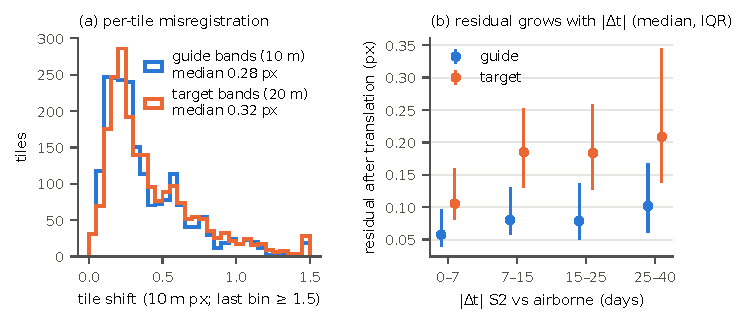
\includegraphics[width=\textwidth]{figures/fig2_geometry.pdf}
\caption{Geometric error of the SEN2NEON reference (2,100 tiles). (a) Magnitude of the per-tile translation between
the degraded reference and Sentinel-2 for the 10\,m guide bands and the 20\,m target bands. (b) Residual
misregistration in $640\times640$\,m blocks after removing the tile translation, by time between acquisitions
(median and interquartile range; 220, 164, 220 and 1,496 tiles per bin).}\label{fig:geometry}
\end{figure}

\paragraph{Contrast.} Fig.~\ref{fig:harmonisation} tests Eq.~\eqref{eq:ols} at the fitting grid of SEN2NEON:
per tile, the ratio of the reference to the interpolated Sentinel-2 standard deviation at 2.5\,m follows their
correlation $R$ in all six target bands (correlation over tiles 0.75--0.81; median ratio minus $R$ between $-0.04$
and $-0.03$), and the tile means of the reference equal those of Sentinel-2 (median absolute difference
$8.4$--$8.8\times10^{-5}$ reflectance across the six target bands). Eq.~\eqref{eq:ols} is an identity only for the
pixel set and interpolated image of the original fit. The ratio lies slightly but systematically below $R$. One
likely reason is that our bilinear interpolation of Sentinel-2 to 2.5\,m is sharper than the SEN2NEON interpolation
(linear interpolation at 1\,m followed by antialiased downsampling), which increases our $\sigma_s$. Differences
between the original fit domain and our tile would add scatter of either sign. Without the pre-harmonised data we
cannot reproduce the fit exactly, so we describe the contrast as consistent with the documented OLS mechanism. At 20\,m against the native Sentinel-2 bands, the median compression factor $\hat a$ of
Eq.~\eqref{eq:gain} is 0.53--0.63 (Table~\ref{tab:errors}; interquartile ranges about 0.4--0.73): the released
reference carries little more than half of the Sentinel-2 contrast, with a large spread between tiles. Registration
alone raises the high-pass correlation between the degraded reference and Sentinel-2 by about 0.03--0.04.

\begin{figure}[t]
\centering
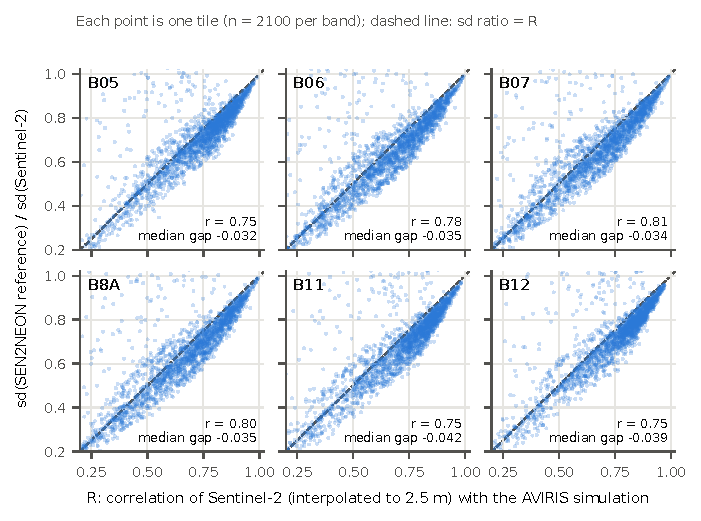
\includegraphics[width=\textwidth]{figures/fig3_harmonisation.pdf}
\caption{The harmonisation regression explains the contrast of the reference. Each point is a tile: ratio of the
standard deviation of the SEN2NEON reference to that of the bilinearly interpolated Sentinel-2 image at 2.5\,m
against their correlation $R$. The dashed line is the prediction of Eq.~\eqref{eq:ols}.}\label{fig:harmonisation}
\end{figure}

%% Sources: results/p6_e0/harmonisation_check_2p5m.md (rows 1-2), results/p6_paper_facts/facts.md (row 3),
%% results/p6_e0/summary.md, radiometry table of the cloud-clean subset (rows 4-5: hp_corr_raw, hp_corr).
\begin{table}[t]
\caption{Reference errors per target band (medians). Rows 1--2: correlation and standard deviation ratio of the
reference and the interpolated Sentinel-2 image at 2.5\,m (2,100 tiles). Row 3: compression factor of the registered
reference against native Sentinel-2 at 20\,m (Eq.~\ref{eq:gain}; the 1,253 tiles of the site split for which it was
computed: 1,019 tiles of the training sites with $|\Delta t|\le40$ days and the 83 validation and 151 test
tiles). Rows 4--5:
high-pass correlation of $D(r)$ with Sentinel-2 at 20\,m before and after registration (1,870 tiles whose Cloud
Score+ value from the SEN2NEON metadata is at most its upper quartile).}\label{tab:errors}
\begin{tabular*}{\textwidth}{@{\extracolsep\fill}lcccccc}
\toprule
 & B5 & B6 & B7 & B8A & B11 & B12 \\
\midrule
$R$ (2.5\,m) & 0.760 & 0.674 & 0.684 & 0.685 & 0.753 & 0.789 \\
$\sigma_{\hat z}/\sigma_s$ (2.5\,m) & 0.729 & 0.650 & 0.658 & 0.655 & 0.711 & 0.750 \\
$\hat a$ (20\,m) & 0.622 & 0.531 & 0.553 & 0.546 & 0.580 & 0.632 \\
HP-corr, as released & 0.792 & 0.721 & 0.723 & 0.724 & 0.807 & 0.832 \\
HP-corr, registered & 0.824 & 0.758 & 0.760 & 0.766 & 0.845 & 0.861 \\
\botrule
\end{tabular*}
\end{table}

\paragraph{Is one compression factor per tile enough?} Three checks support Eq.~\eqref{eq:gain}. In E1-R, where the true
compression $m$ is known, $\hat a$ recovered it closely: over 1,524 validation tile-bands, $\hat a/m$ had a median
of 0.999 and a 5--95\,\% range of 0.996--1.002 (medians of $\hat a$ 0.740--0.768 against $m$ 0.740--0.770),
although $R$ was about 0.92 there; the gain to invert is $m$, which explains
why $\hat a$ is lower than $R$ on real data as well. Second, we computed the same standard-deviation ratio, $\operatorname{sd}B(D(\rreg))/\operatorname{sd}B(x)$, for
band-pass components $B$ given by differences of Gaussian low-passes ($\sigma$ = 20--40, 40--80 and 80--160\,m), on
the pixels whose whole filter footprint is valid, and divided it by $\hat a$ of the same tile and band. On real data
(the 521 tiles of domain R; scales without enough valid pixels are skipped) the median
ratio was 0.97, 1.02 and 1.02 (tile-bootstrap 95\,\% CIs 0.96--0.99, 1.01--1.03 and 1.01--1.03; per-tile
interquartile ranges about 0.88--1.10; per band, 0.95--0.99 at the finest scale and 1.01--1.03 at the others); in
domain S, where the true gain is the same at every scale by construction, the measured medians were 0.97, 0.99 and
1.00. The drop at the finest scale is therefore a property of the measurement (noise and aliasing in the 20\,m input),
and the real gain departs from the measurement effect by at most about 3\,\% at the tested scales. Third, the 10\,m
bands offer a positive control with real truth: SEN2NEON harmonises them in the same way, and Sentinel-2 observes
them at 10\,m. We applied the same registration (with the guide-band shift) and compensation (Eq.~\ref{eq:gain} on
the 10\,m grid) to the reference of B2, B3, B4 and B8 and compared each version with the Sentinel-2 bands with the
high-pass of $\sigma=20$\,m used for all evaluations (519 tiles, 40 sites; medians over tiles and bands). The
frequency bands of estimation and evaluation hardly overlap: where the high-pass passes half of the signal
(0.0094 cycles/m), the 60\,m low-pass used for $\hat a$ transmits 0.2\,\%. The estimate and the evaluation still
use the same Sentinel-2 image, so the control is not fully independent. The released
reference carried 0.62 of the Sentinel-2 high-pass amplitude; registration raised the high-pass correlation from
0.83 to 0.87 and lowered the edge error from 1.27 to 1.13 pixels; the compensation raised the amplitude to 0.82
(0.78--0.86 per band; median of site medians 0.81, site-bootstrap CI 0.77--0.83, higher at all 40 sites) and the
HP-PSNR by 0.8\,dB, improving it at 33 of the 40 sites. The compensation thus recovers most, but not all, of the
Sentinel-2 detail amplitude; the remaining shortfall at the finest scales is
consistent with point-spread-function differences, residual misregistration and Sentinel-2 noise.

\section{Results: controlled study}\label{sec:res-controlled}

\paragraph{Misregistration (E1).} Table~\ref{tab:e1} shows that misregistration of the size measured in E0 barely
affects training: no method lost more than 0.003 HP-corr from S0 to S2, and only the stress scenario S3 cost
Naive-L1 and FDL about 0.008--0.010. By the H2 rule, Shift-L1 was selected: FDL was ineligible (edge error 0.644 against the limit 0.597), and among the
eligible losses Shift-L1 had the highest HP-corr in S2, above Naive-L1, Reg-L1, CoBi, PISR and both P6 forms by
0.0013--0.0112 (all Holm-adjusted tile-bootstrap $p<0.001$; because E1 has only two evaluation sites, these $p$-values describe
tile-level variability and are not site-level evidence). It was the best loss in
all four scenarios, ahead of Reg-L1 by $0.0017\pm0.0005$ HP-corr in S2 (mean $\pm$ sd of three paired seeds). Distillation
did not help: PISR matched Reg-L1, and P6 was below it ($-0.0013\pm0.0004$ in S2). CoBi and FDL, which had to be
adapted to six bands, were clearly worse. The largest effect in Table~\ref{tab:e1} is not the corruption but the
supervision scale: training only at the reduced scale (Wald) gave, in S0--S2, an HP-corr
0.039--0.055 below the supervised methods and an HP-PSNR 4.3--6.2\,dB lower. The H2 selection of Shift-L1 rests on
descriptive tile-level intervals (Section~\ref{sec:method-training}).

%% Source: runs/p6_e1/summary_eval.md (seed 0, 181 tiles, tile means) and its seed replication table.
\begin{table}[t]
\caption{E1 on domain S: HP-corr against the clean target (tile means over 181 tiles of two validation sites,
seed 0). S0: clean target; S1: tile shift; S2: realistic (shift, non-rigid, change); S3: stress. Bold: best per
scenario. Edge S2: edge-position error in S2, used by the H2 rule. Three-seed means in S2: Shift-L1 0.9696, Reg-L1 0.9679, P6 (global) 0.9666, Naive-L1 0.9648 (seed sd
0.0001--0.0005).}\label{tab:e1}
\begin{tabular*}{\textwidth}{@{\extracolsep\fill}lccccc}
\toprule
Method & S0 & S1 & S2 & S3 & Edge S2 (px) \\
\midrule
Wald & 0.9141 & 0.9140 & 0.9138 & 0.9141 & 0.834 \\
Naive-L1 & 0.9670 & 0.9646 & 0.9644 & 0.9587 & 0.570 \\
Reg-L1 & 0.9667 & 0.9687 & 0.9679 & 0.9647 & 0.547 \\
Shift-L1 & \textbf{0.9685} & \textbf{0.9694} & \textbf{0.9692} & \textbf{0.9662} & 0.542 \\
CoBi & 0.9570 & 0.9581 & 0.9580 & 0.9592 & 0.588 \\
FDL & 0.9537 & 0.9540 & 0.9524 & 0.9439 & 0.644 \\
PISR & 0.9668 & 0.9682 & 0.9679 & 0.9633 & 0.542 \\
P6 (local) & 0.9662 & 0.9674 & 0.9672 & 0.9631 & 0.547 \\
P6 (global) & 0.9659 & 0.9673 & 0.9669 & 0.9627 & 0.547 \\
\botrule
\end{tabular*}
\end{table}

\paragraph{Harmonisation, training (E1-R).} Training on the harmonised target lowered the structural quality of the
predictions, scored against the true target (Table~\ref{tab:e1r}): HP-corr fell from 0.9768 to 0.9693 and the edge
error rose by 11\,\%; the difference had the same sign at both sites and in all three seeds (HP-corr $-0.003$ at
one site and $-0.011$ to $-0.012$ at the other). Inverting the harmonisation with
Eq.~\eqref{eq:gain} recovered the clean-target HP-corr and brought HP-PSNR and edge error to within 0.05\,dB and
0.001 pixels of it. Contrary to our expectation, the detail amplitude did not fall to the compression factor
($m\approx0.75$) but stayed near 1.05: the LFC ties the output to the full-contrast input, and the conflict between
input and compressed target appears as distorted rather than attenuated detail. Reg-HP trained on the uncorrected
$y_h$ was the best model, above L1 on the clean target in both HP-corr and HP-PSNR.

%% Source: runs/p6_e1r/analysis/summary.md (part A; reg_hp_h with the corrected loss); site means.
\begin{table}[t]
\caption{E1-R on domain S: effect of the harmonisation on training, scored against the true target (two validation
sites, mean of site means; mean $\pm$ sd over three seeds).}\label{tab:e1r}
\begin{tabular*}{\textwidth}{@{\extracolsep\fill}lcccc}
\toprule
Training target & HP-PSNR (dB) & HP-corr & HP-gain & Edge error (px) \\
\midrule
L1, true $y$ & $56.63\pm0.03$ & $0.9768\pm0.0003$ & $1.086\pm0.002$ & $0.492\pm0.001$ \\
L1, harmonised $y_h$ & $55.79\pm0.07$ & $0.9693\pm0.0002$ & $1.057\pm0.004$ & $0.544\pm0.002$ \\
L1, inverted $y_{\mathrm{inv}}$ & $56.59\pm0.01$ & $0.9768\pm0.0002$ & $1.089\pm0.001$ & $0.491\pm0.000$ \\
Reg-HP, harmonised $y_h$ & $56.89\pm0.04$ & $0.9807\pm0.0001$ & $1.084\pm0.003$ & $0.470\pm0.001$ \\
\botrule
\end{tabular*}
\end{table}

\paragraph{Harmonisation, evaluation (E1-R).} The more serious effect is on evaluation (Fig.~\ref{fig:rankflip}).
When the same 22 models were scored against the harmonised reference instead of the true one, their ranking by
HP-PSNR changed substantially (Kendall $\tau=0.53$; tile-bootstrap interval 0.47--0.63): the model trained on the harmonised
target moved from rank 16 to rank 1, and FDL, whose outputs are smooth, from rank 18 to rank 4. A compressed
reference rewards predictions with compressed detail. The 22 models include S0 and S2 versions of the same methods;
with one model per method (13 models) the agreement was lower still ($\tau=0.21$, interval 0.08--0.33). These
$\tau$ values describe the given model sets; the concrete rank changes matter more than their exact value. Against the
inverted reference the ranking was preserved ($\tau=1.00$, interval 0.99--1.00), as expected from the near-exact gain
recovery above; the ranking by HP-corr, which is invariant to the gain, was identical for all three references.
Ranks are by tile means with seeds averaged (runs/p6\_e1r/analysis/tau\_ci.md in the released material).

\begin{figure}[t]
\centering
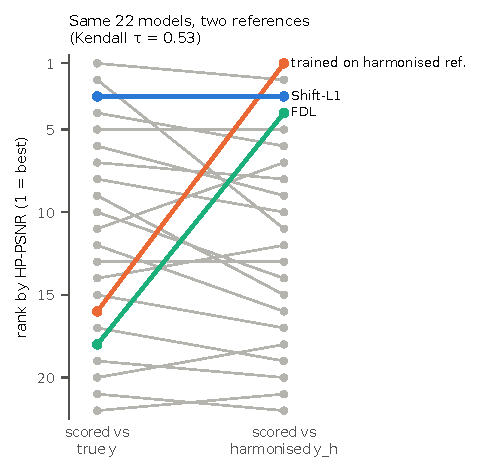
\includegraphics[width=0.62\textwidth]{figures/fig4_rank_flip.pdf}
\caption{Ranking of 22 models by HP-PSNR on domain S when scored against the true target (left) and against the
target harmonised as in SEN2NEON (right). Highlighted: the model trained on the harmonised target, FDL and
Shift-L1.}\label{fig:rankflip}
\end{figure}

\section{Results: real data}\label{sec:res-real}

\paragraph{Corrections.} Training on corrected references matters on real data (Table~\ref{tab:e2},
Fig.~\ref{fig:e2}). Reg-L1 exceeded Naive-L1 by 0.043 HP-corr (CI 0.026 to 0.065; higher at all nine sites) and reduced the edge
error by 0.12 pixels; registration alone (Reg-L1 without gain against Naive-L1) contributed 0.011 (eight of nine sites) and changed the
learned detail amplitude (HP-gain against $y_c$) only from 0.61 to 0.64, whereas the gain compensation alone (Reg-L1
against Reg-L1 without gain) contributed 0.032 (CI 0.021 to 0.043; all nine sites) and raised the HP-gain from 0.64
to 0.99 (an amplitude measured against our own calibration). Training on the compressed references also degraded the consistency with the observed 20\,m bands:
the full-resolution PSNR of Naive-L1 was 38.9\,dB, with a contrast of $D(\hat y)$ of 0.82 of $x$, against 46.0\,dB
and 0.95 for Reg-L1 (all nine sites), because the approximate LFC does not fully undo a compressed output. For scale,
bicubic upsampling of $x$ reached an HP-corr of 0.733, below every supervised method and the Wald model. HP-corr
does not depend on our gain estimate; these differences arise because a compressed training target changes the
detail the network learns, as in E1-R. They persist when the models are scored against the 10\,m aggregate of the reference as released, without
registration or gain compensation (Table~\ref{tab:e2}, last column): the order of the methods by
HP-corr is unchanged, and Reg-L1 still exceeds Naive-L1 by 0.035 (CI 0.019 to 0.053). Scored against the registered reference with
the contrast as delivered, the HP-PSNR ranking reverses at the bottom: Naive-L1 and Reg-L1 without gain obtained the
highest HP-PSNR of all methods (44.5\,dB against 42.0\,dB for Reg-L1), while they are the two lowest supervised
methods by HP-corr. The HP-PSNR rankings against the two references agreed only weakly (Kendall
$\tau=0.33$, CI 0.17--0.56; one-sided permutation test of agreement beyond chance, $p=0.13$ with 5,000
permutations). Between $y_c$ and $\rreg$ the rankings by HP-corr, edge error and HP-gain were identical; HP-corr is
gain-invariant, the edge metric is insensitive to a positive global gain, and for HP-gain the agreement is empirical.
Against the unregistered reference $r$, the HP-corr and HP-gain rankings were also identical and the edge-error
ranking nearly so ($\tau=0.94$), as the edge metric is sensitive to registration.

%% Sources: runs/p6_e2/analysis/summary.md, runs/p6_e2_posthoc/analysis/summary.md (site means, test sites) and
%% runs/p6_e2/analysis/gpt_revision_summary.md (Bicubic row, Full res. column).
\begin{table}[t]
\caption{E2 on the nine real test sites (151 tiles). Learned methods were run with three seeds (mean over seeds;
largest seed sd: HP-corr 0.003, HP-PSNR 0.17\,dB, edge 0.015\,px, HP-gain 0.015, full-resolution PSNR 0.15\,dB, Wald
fidelity 0.49\,dB); Bicubic is deterministic. HP-PSNR, HP-corr, edge and HP-gain
against the corrected reference $y_c$; HP-PSNR($\rreg$) against the registered reference with the contrast as
delivered (HP-corr against $\rreg$ equals HP-corr against $y_c$); HP-corr($r$) against the 10\,m aggregate of the
reference as released. Full res.: PSNR of $D(\hat y)$ against the observed 20\,m bands. Wald: reduced-scale fidelity.
Bicubic: $\hat y=U(x)$, no learning. $^\dagger$Exploratory, post hoc ($\lambda_W=30$ chosen on validation sites).}\label{tab:e2}
\footnotesize\setlength{\tabcolsep}{2.5pt}
\begin{tabular*}{\textwidth}{@{\extracolsep\fill}lcccccccc}
\toprule
 & \multicolumn{4}{c}{against $y_c$} & $\rreg$ & $r$ & \multicolumn{2}{c}{consistency} \\
\cmidrule(lr){2-5}\cmidrule(lr){6-6}\cmidrule(lr){7-7}\cmidrule(lr){8-9}
Method & HP-PSNR & HP-corr & Edge & HP-gain & HP-PSNR & HP-corr & Full res. & Wald \\
\midrule
Bicubic & 40.01 & 0.7326 & 1.693 & 0.75 & 42.59 & 0.7026 & 45.38 & -- \\
Wald & 37.22 & 0.7753 & 1.387 & 1.57 & 36.11 & 0.7261 & 56.88 & 48.07 \\
Naive-L1 & 40.63 & 0.7865 & 1.389 & 0.61 & 44.51 & 0.7483 & 38.85 & 46.63 \\
Reg-L1, no gain & 40.84 & 0.7974 & 1.345 & 0.64 & 44.50 & 0.7553 & 39.06 & 46.73 \\
B-sim & 39.96 & 0.8114 & 1.279 & 1.26 & 38.94 & 0.7621 & 51.21 & 45.43 \\
B-sim+FT & 41.42 & 0.8252 & 1.278 & 1.01 & 41.75 & 0.7791 & 46.01 & 47.57 \\
Shift-L1 & 41.57 & 0.8268 & 1.268 & 0.99 & 41.89 & 0.7813 & 45.14 & 47.62 \\
P6 & 41.72 & 0.8287 & 1.261 & 0.98 & 42.10 & 0.7834 & 45.46 & 47.58 \\
Reg-L1 & 41.60 & 0.8292 & 1.271 & 0.99 & 42.00 & 0.7834 & 46.03 & 47.69 \\
Reg-HP ($\lambda_W=1$) & 41.45 & \textbf{0.8364} & \textbf{1.228} & 1.12 & 40.65 & \textbf{0.7894} & 47.84 & 42.00 \\
\midrule
Reg-HP ($\lambda_W=30$)$^\dagger$ & 41.38 & 0.8354 & 1.233 & 1.13 & 40.53 & 0.7886 & 48.72 & 47.47 \\
\botrule
\end{tabular*}
\end{table}

\begin{figure}[t]
\centering
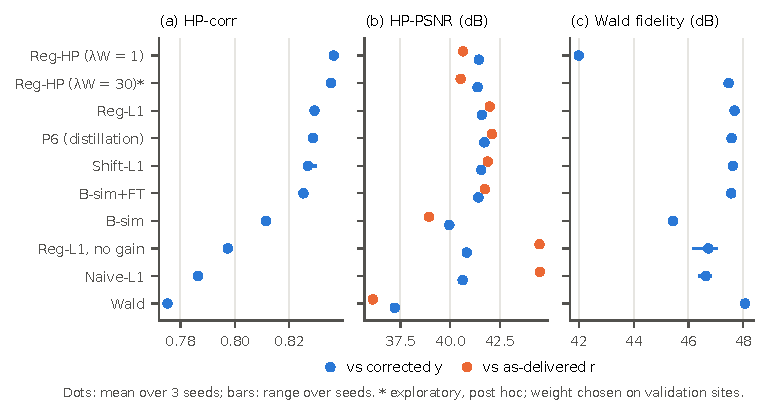
\includegraphics[width=\textwidth]{figures/fig5_e2.pdf}
\caption{E2 on the nine real test sites. (a) HP-corr against the corrected reference; (b) HP-PSNR against the
corrected reference and against the reference with the contrast as delivered; (c) reduced-scale (Wald) fidelity. Dots: mean
over three seeds; bars: range over seeds.}
\label{fig:e2}
\end{figure}

\paragraph{Strategies.} Intervals in this paragraph are hierarchical-bootstrap intervals; site counts refer to
the nine paired site differences. With the corrected reference, Reg-L1, Shift-L1 and P6 were close. Shift-L1, the best loss in
simulation, did not improve over Reg-L1 on real data ($-0.0024$ HP-corr, CI $-0.0068$ to $0.0023$, although lower at all nine
sites): after per-tile registration there is little misalignment left for it to absorb. We did not detect an improvement of P6 over Reg-L1 ($-0.0005$, CI $-0.0042$ to $0.0048$; lower at eight of nine
sites). Nor did we detect a benefit of simulated data: B-sim alone was 0.018 below Reg-L1 (CI
0.010 to 0.026), B-sim+FT remained below Reg-L1 ($-0.0041$, CI $-0.0085$ to $-0.0017$), and it did not
improve over Shift-L1 trained from scratch, the loss of its second stage ($-0.0017$, CI $-0.0074$ to $0.0015$). This
compares a curriculum of 10,000 simulated plus 10,000 real steps with 20,000 real steps; it does not isolate the
effect of pre-training at an equal number of real steps. Reg-HP gave the best structure, with
HP-corr $+0.0071$ over Reg-L1 (CI 0.0016 to 0.0162; higher at seven of nine sites, permutation $p=0.03$) and the
lowest edge error, with the HP-PSNR difference to Reg-L1 not resolved. Its full-resolution consistency was also the
highest among the models trained on real references (47.8 against 46.0\,dB for Reg-L1; paired difference 1.8\,dB,
t-interval 0.8 to 2.8, higher at eight of nine sites, exact sign-flip $p=0.01$; higher than Shift-L1 at all nine
sites), whereas its reduced-scale fidelity was the lowest (42.0\,dB). The Wald-only model and B-sim reproduce the
observed bands even more closely (56.9 and 51.2\,dB) but with much lower structural fidelity. Fig.~\ref{fig:qualitative} shows a typical test crop: the reference as released has visibly less contrast
than Sentinel-2, Naive-L1 reproduces this flat appearance, the Wald model adds spurious texture, and the methods
trained on the corrected reference recover the field boundaries and small structures.

\begin{figure}[t]
\centering
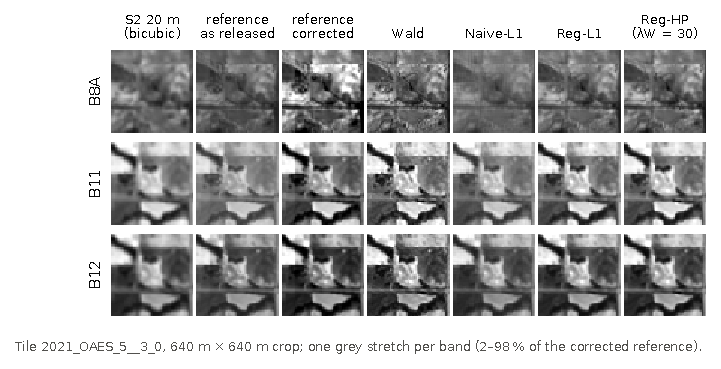
\includegraphics[width=\textwidth]{figures/fig6_qualitative.pdf}
\caption{Test crop of $640\times640$\,m at OAES (bands B8A, B11, B12; seed-0 models). The tile was chosen by a rule
fixed before viewing: among test tiles in the top quartile of reference detail, the one whose Reg-L1 HP-corr is
closest to the median of that group; the crop is the window with the most reference detail. One grey stretch per
band, from the corrected reference.}\label{fig:qualitative}
\end{figure}

\paragraph{Pre-specified hypotheses.} The intervals in this paragraph are the pre-specified site bootstrap of
seed-averaged site means. H1 was not supported. Reg-HP beat Wald on both co-primary endpoints
(HP-PSNR $+4.23$\,dB, CI 3.52 to 5.12; HP-corr $+0.061$, CI 0.052 to 0.072), but its reduced-scale (Wald) fidelity was
6.1\,dB lower (CI $-6.7$ to $-5.5$; hierarchical bootstrap: 3.55 to 5.05\,dB, 0.052 to 0.071 and $-6.7$ to
$-5.5$\,dB), far beyond the 0.10\,dB margin. This criterion concerns the 40$\to$20\,m synthesis test, not the
consistency of the 10\,m output with the observed bands, for which Reg-HP was better than all other models trained
on real references. In hindsight the margin, set against the Wald model itself, was too strict: every other method also lost
0.4--2.6\,dB on this measure. H3 was not supported:
P6 beat B-sim+FT on both endpoints (step 1; HP-PSNR $+0.30$\,dB, CI 0.01 to 0.84; HP-corr $+0.0035$, CI 0.0002 to
0.0091; hierarchical bootstrap 0.01 to 0.94 and 0.0001 to 0.0108; at site level, HP-corr was higher at seven of nine sites,
permutation $p=0.07$), but step 2 failed: P6 was below Reg-HP in HP-corr
($-0.0076$, CI $-0.0130$ to $-0.0029$, Holm-adjusted $p<0.001$) and the HP-PSNR difference was not statistically resolved ($+0.28$\,dB, CI $-0.26$ to $0.75$, Holm-adjusted
$p=0.28$). These $p$-values are two-sided bootstrap tail shares (twice the smaller
share of bootstrap differences on either side of zero), Holm-adjusted over the two endpoints; with nine sites they
are approximate. As a sensitivity analysis we therefore also applied exact two-sided sign-flip tests to the nine
paired site differences (512 sign patterns). They confirm the verdicts on H1 (both co-primary endpoints favour
Reg-HP at all nine sites, $p=0.004$; reduced-scale fidelity lower at all nine sites) and on H3 step 2 (HP-corr lower
at all nine sites, Holm-adjusted $p=0.008$), but they do not confirm step 1: P6 was better than B-sim+FT at six and
seven of nine sites ($p=0.055$ and $0.066$, Holm-adjusted 0.11). The hierarchical bootstrap gives the same verdicts as
the pre-specified analysis. Under every analysis H3 is not supported.

\paragraph{Exploratory, post hoc: Wald weight for Reg-HP.} The low reduced-scale fidelity of Reg-HP suggested that
its normalised high-pass loss dominates the Wald loss. After seeing the E2 results we therefore ran Reg-HP with
$\lambda_W\in\{3,10,30\}$ (seed 0) and fixed a selection rule before evaluating them: on the four validation sites,
keep the weights whose reduced-scale fidelity is within 0.5\,dB of Reg-L1 and choose the highest HP-corr. Only
$\lambda_W=30$ qualified (47.31 against 47.52\,dB for Reg-L1; $\lambda_W=3$ and 10 gave 42.98 and 45.21\,dB). On the
test sites, with three seeds, it kept the structural advantage of Reg-HP over Reg-L1 (HP-corr $+0.0061$, CI 0.0010
to 0.0141; edge error $-0.038$\,pixels, CI $-0.086$ to $-0.012$; hierarchical bootstrap as for E2) at a reduced-scale
fidelity 0.22\,dB below Reg-L1 (CI $-0.46$ to $-0.04$) instead of 5.7\,dB, with the HP-PSNR difference not resolved
and a full-resolution consistency of 48.7\,dB. This result is exploratory: it was not
pre-specified, it does not change the verdict on H1, and it should be confirmed on independent sites.

\section{Discussion}\label{sec:discussion}

\paragraph{Implications for training.} The two corrections matter, and they are simple. Per-tile
registration and the inversion of the harmonisation gain together improved the structural agreement with the
reference by far more than any choice of loss or training scheme, and the improvement does not depend on scoring
against the corrected reference. Once they are applied, shift-tolerant losses did not improve the results, consistent with the small remaining
misregistration. A high-pass loss that ignores the gain of the reference gave the best structure in
simulation and on real data and, among models trained on real references, the best consistency with the observed
20\,m bands; as pre-specified it had low
reduced-scale fidelity (H1 not supported), which our exploratory analysis suggests a stronger reduced-scale term
restores. This recommendation rests on secondary and exploratory results and should be confirmed on independent
sites. For our student and protocol, the reduced-scale (Wald) training that is common practice was the
weakest learned option in both domains; compared with the methods trained on corrected references the gap was about
0.05 HP-corr: the 40$\to$20\,m proxy does not substitute for a 10\,m reference.

\paragraph{Why the complex methods did not help.} Contextual and frequency losses were designed for large
misalignments in natural images and rely on pretrained RGB features; our six-band adaptations, with small residual
shifts, cost more than they gained in simulation, and we did not carry them to real data. This concerns our
adaptations under a small tuning budget, not contextual or frequency losses in general. Privileged distillation assumes that the teacher holds information the student cannot obtain
otherwise. Here the teacher sees an encoding of the reference, but the student is already supervised by the same
reference; the distillation term then adds a second, noisier path to the same information. This held although PISR
and P6 received an additional 30,000 teacher steps and a teacher-initialised student. Simulation-only training
suffered from the gap between simulated and real Sentinel-2 inputs; under a fixed budget of 20,000 student steps,
10,000 simulated plus 10,000 real steps did not improve over 20,000 real steps with the same loss.

\paragraph{Consequences for SEN2NEON users.} Three practical recommendations follow. (i) Exclude the 131 tiles with
resampled 20\,m bands. (ii) Register each tile and invert the harmonisation gain before training; we release the
shifts, gains and corrected references. (iii) Report an amplitude-invariant metric such as HP-corr next to
PSNR-type metrics, together with the full-resolution consistency $D(\hat y)$ against $x$: against the released
reference, amplitude-sensitive metrics reward low-contrast outputs and can change conclusions, whereas HP-corr is
unaffected by the gain but blind to amplitude errors. The SEN2NEON authors evaluate the consistency of SR
outputs with the low-resolution input after histogram matching \citep{donike2026sen2neon}, which is not affected;
the issue concerns any use of the 2.5\,m reference as a target. The mechanism is general: any reference built by
regressing a coarse sensor on a sharp one and keeping the fitted values inherits the compression, and a symmetric
fit or the inversion of Eq.~\eqref{eq:gain} avoids it. Whether full Sentinel-2 contrast is the right target depends
on the use: for SR of Sentinel-2 it is, by definition of the task; for studies of the airborne signal itself, the
unscaled airborne image would be preferable.

\paragraph{Limitations.} All sites are in the United States, and the test set has nine sites in a single split;
site-level intervals are wide for small differences, and a different split might reorder close methods. Domain S is
a simulation: its corruption pipeline interpolates the target, which made S1 and S2 score slightly above S0 in E1,
so only comparisons within a scenario are meaningful; E1 has only two evaluation sites. Our gain estimate assumes
that the low-frequency contrast of Sentinel-2 is correct and that surface change within seven days is small, and
$y_c$ remains a model-based calibration. The aggregation kernel matches the Sentinel-2 MTF only at Nyquist, so the
effective point-spread function of the corrected reference may still differ from that of a true 10\,m Sentinel-2
image; the MTF sensitivity test covers shifts and gains, not this effect on training and evaluation. The gain
compensation also amplifies any high-frequency noise of the reference, and on the 10\,m bands it recovered most but
not all of the Sentinel-2 detail amplitude. Three of the four auxiliary weights tuned in E1 lay on the boundary of
their grid, and the grid was not extended by our pre-specified rule; CoBi and FDL had to be adapted to six bands and
were not run on real data. Budgets were matched in student steps, not in total computation (Table~\ref{tab:methods}); in particular, B-sim+FT
received half of the real-data steps of the other methods. The Wald weight of
Reg-HP was chosen after seeing the E2 results, on validation sites. An implementation error in the first version
of Reg-HP (the prediction scale was detached from the gradient, which collapsed the detail amplitude) was found
after the first seed of E2; that run and the three E1-R Reg-HP runs were discarded and rerun with the corrected loss
before any other Reg-HP run, and only corrected runs are reported. The dated amendment in the E2 configuration
records the change, the erroneous run is archived and labelled invalid, and the method and the hypotheses were not
changed; H1 was thus tested with the corrected implementation after a dated bug fix. After completion of the pre-specified E2 tests, the initially
single-seed secondary methods (Naive-L1, Reg-L1 without gain and B-sim) were rerun with two additional seeds; the
configuration records this amendment.

\section{Conclusion}\label{sec:conclusion}

The first real-reference benchmark for the 20\,m bands of Sentinel-2 carries systematic errors that matter for deep
learning: a per-tile misregistration, a contrast compression by the harmonisation regression, and resampled inputs
in part of the tiles. Training on the reference as released lowers structural fidelity, and evaluating against it
with amplitude-sensitive metrics can change the ranking of methods. Per-tile registration and one compression
factor per tile and band compensate most of the problem under the assumed degradation model, as a positive control
on the 10\,m bands confirms; with them, a gain-invariant high-pass loss gave the best structure and, among models trained on real references, the best consistency
with the observed bands (with a caveat on reduced-scale fidelity that an exploratory analysis addressed), whereas shift-tolerant losses,
privileged distillation and, within a fixed step budget, simulation pre-training did not improve on plain L1. We hope that the
corrected references and the protocol make SEN2NEON a more reliable basis for both training and evaluation.

\backmatter

\bmhead{Acknowledgements}
We thank the authors of SEN2NEON for releasing the dataset under an open licence, and NEON for the airborne
observations.

\section*{Declarations}

\begin{itemize}
\item Funding: The authors did not receive support from any organization for the submitted work.
\item Competing interests: The authors declare no competing interests.
\item Use of AI tools: The authors used Anthropic Claude to assist in writing the experiment and analysis code; all
code was reviewed and verified by the authors. Claude also assisted in drafting the text from the authors' results
and outline, and AI tools were used to correct spelling and grammar; the authors revised and verified all text and
numbers. The study concept and the analysis and interpretation of the results are the authors' own.
\item Data availability: SEN2NEON is available under CC-BY-4.0 \citep{donike2026sen2neon}. The derived data are
released under the same licence, with attribution: the per-tile shifts, compression factors, site split and all
per-run results are in the code repository (below); the corrected references of domain~R and the weights of all
reported models (about 5\,GB) are deposited as a Zenodo dataset linked from the repository and will be public at the
latest on publication.
\item Code availability: The code, the configurations with the pre-specified analysis rules and their freeze dates
(E1: 12 October 2026; E2: 14 October 2026, with a dated amendment on 15 October 2026 for the Reg-HP implementation
fix; post hoc: 17 October 2026), the analysis outputs and the tests are available at \url{https://github.com/vubcfe/s2sr-imperfect-references} and archived on Zenodo
(\url{https://doi.org/10.5281/zenodo.23448595}).
\item Author contributions: C.V.B.: conceptualization, methodology, software, investigation, formal analysis,
writing (original draft). H.-A.-V.N.: validation, formal analysis, writing (review and editing). All authors read
and approved the final manuscript.
\end{itemize}


\begin{appendices}

\section{Auxiliary losses and weights}\label{app:losses}

All weights below were chosen on the domain-S tuning sites (CLBJ, DSNY) in scenario S2 with one third of the steps,
one weight at a time from a three-value grid ($\times0.1$, $\times1$, $\times10$ of a default), by the mean HP-corr;
the grid was not extended afterwards. Every loss is added to $\mathcal{L}_W$ ($\lambda_W=1$) and, except CoBi and
FDL, to the L1 loss of the method.

\paragraph{CoBi.} Contextual bilateral loss \citep{zhang2019zoom} on $5\times5$ patches of the six target bands
(150-dimensional patch vectors), cosine distance plus $w_s=0.05$ times the spatial distance in pixels, computed on
1,024 random positions per patch; weight 10 (upper end of the grid).

\paragraph{FDL.} Frequency distribution loss \citep{ni2024fdl}: sliced Wasserstein distances between the
distributions of the Fourier amplitude and phase of features, here of a frozen Wald-trained student instead of VGG; weight 0.1 (lower end of the grid).

\paragraph{PISR.} Teacher: an encoder of the reference (four convolutions with kernels 5, 5, 3 and 3, the second strided
by two, with PReLU between them) and a decoder with the student's architecture, trained for 30,000 steps with
$\lVert T(E(y), g)-y\rVert_1 + 10^{-4}\lVert E(y)-D(y)\rVert_1$. The student is initialised with the decoder and
trained with L1 plus variational information distillation \citep{ahn2019vid} on the outputs of its last two
residual blocks: an estimator (two branches of $1\times1$ convolution, PReLU, $1\times1$ convolution; softplus on
the scale) predicts a Laplace location $\mu$ and scale $b$ of each teacher feature from the student feature, and
the loss is the mean of $\log b + |h^T-\mu|/b$; weight $10^{-5}$ (the grid was flat).

\paragraph{P6.} PISR with the distillation applied to the high-frequency part of the features
($h - \mathrm{AvgPool}_{5\times5}(h)$), plus a patch-contrastive term. Student and teacher features are projected by
two-layer $1\times1$ heads to 128 dimensions and normalised. For each tile, 256 anchor positions are drawn; the
positive is the teacher feature at the same position shifted by $s$, with $s$ chosen per anchor within one feature
pixel (local form) or once per tile as the shift among the nine candidates that maximises the mean anchor--positive
similarity (global form). Negatives are 256 positions of the same tile at least 8 pixels away and 256 positions of
the other tiles of the batch; negatives whose teacher feature has a cosine similarity above 0.9 with the positive
are dropped. The loss is InfoNCE with temperature 0.1; weight $10^{-4}$ (lower end of the grid), distillation weight
$10^{-5}$.

\end{appendices}

\bibliography{refs}

\end{document}
